% !TeX program = lualatex
% ================================================================
% Polish Tier 3 Vocabulary Version of PureRatioCrossTopics
%
% Generated by the server using the following settings:
%
%   language            Polish (pol)
%   text direction      left to right
%   font                Noto Serif
%   fallback font       Noto Serif
%   built from          latex/worksheets/ratioAndProportion/crossTopic/pureRatioCrossTopics.tex
%   vocabulary key      latex/worksheets/ratioAndProportion/crossTopic/pureRatioCrossTopics/L2/pol/pureRatioCrossTopics_polishKey.tex
%   tier 3 vocabulary   green   RGB 0 128 0
%   English text        black   RGB 0 0 0
%   Polish text         purple  RGB 112 48 160
%   layout macros       version 3
%
% Please don't edit any information in this comment block - the server
% compares it against the current settings and rebuilds this file when
% they differ, so changes here would be overwritten. However, feel free
% to make updates to the LaTeX below if you want to edit it.
% ================================================================

\documentclass[12pt,a4paper]{article}
% ================================================================
% Copied from the English sheet this was translated from, so that
% anything it sets up for itself still works here
% ================================================================
\usepackage{amsmath} % For advanced math formatting
\usepackage{enumitem} % For customising lists
\usepackage{tikz} % For drawing diagrams
\usepackage{geometry} % For adjusting page margins
\geometry{margin=1in}

\title{Ratio Extension Problems}
\date{}

% Characters this language's font has not got are borrowed from another,
% rather than being silently dropped - see docs/translated-sheet-latex.md
\directlua{%
  if luaotfload and luaotfload.add_fallback then
    luaotfload.add_fallback("eallatinfallback",
      { "Noto Serif:mode=harf;" })
  else
    tex.error("this luaotfload is too old to register a fallback font")
  end
}
\usepackage[english]{babel}
\babelprovide[import]{polish}
\babelfont[polish]{rm}[Renderer=Harfbuzz, BoldFont={Noto Serif}, ItalicFont={Noto Serif}, BoldItalicFont={Noto Serif}, RawFeature={fallback=eallatinfallback}]{Noto Serif}
\babelfont[polish]{sf}[Renderer=Harfbuzz, BoldFont={Noto Serif}, ItalicFont={Noto Serif}, BoldItalicFont={Noto Serif}, RawFeature={fallback=eallatinfallback}]{Noto Serif}
\newcommand{\ealtext}[1]{\foreignlanguage{polish}{#1}}
\newcommand{\ealtextblock}[1]{{\raggedright\foreignlanguage{polish}{#1}\par}}
% ================================================================
% EAL layout helpers
% ================================================================
\usepackage{xcolor}

\definecolor{ealkeycolour}{RGB}{0,128,0}
\definecolor{ealenglish}{RGB}{0,0,0}
\definecolor{ealtwocolour}{RGB}{112,48,160}

\newsavebox{\ealboxen}
\newsavebox{\ealboxtr}
\newlength{\ealglosswd}
\newlength{\ealglossraise}
\setlength{\ealglossraise}{1.15em}

% a tier 3 word, in English and in translation alike
\newcommand{\ealkey}[1]{\textcolor{ealkeycolour}{#1}}
\newcommand{\ealkeytr}[1]{\textcolor{ealkeycolour}{\ealtext{#1}}}

% One translated word above one English word. Built from kernel
% primitives, never a tabular, which would break wherever the sheet
% loads array, booktabs or tabularx. The box is as wide as the wider of
% the two, so a long translation pushes its neighbours aside instead of
% overlapping them, and it claims its full height so a table row or a
% TikZ node makes room for it.
\newcommand{\ealgloss}[2]{%
  \sbox{\ealboxen}{\ealkey{#1}}%
  \sbox{\ealboxtr}{\small\textcolor{ealtwocolour}{\ealtext{#2}}}%
  \setlength{\ealglosswd}{\wd\ealboxen}%
  \ifdim\wd\ealboxtr>\ealglosswd\setlength{\ealglosswd}{\wd\ealboxtr}\fi
  \leavevmode
  \makebox[\ealglosswd][c]{%
    \makebox[0pt][c]{\usebox{\ealboxen}}%
    \makebox[0pt][c]{\raisebox{\ealglossraise}{\usebox{\ealboxtr}}}%
  }%
}

% opens up line spacing around a block of glosses, so the raised
% translations sit clear of the line above
\newenvironment{ealglossed}{\par\linespread{2.1}\selectfont\ignorespaces}{\par}

% a whole translated sentence above its English counterpart. block level,
% so it does not belong inside a tabular cell
\newcommand{\ealpara}[2]{%
  \par\addvspace{0.5\baselineskip}%
  {\color{ealtwocolour}\ealtextblock{#1}}%
  \penalty200
  {\color{ealenglish}#2\par}%
  \addvspace{0.5\baselineskip}%
}

\begin{document}

\maketitle

\begin{ealglossed}
\section*{\ealgloss{Simplifying}{Upraszczanie} \ealgloss{Ratios}{stosunków} Past}
\end{ealglossed}

\begin{ealglossed}
\emph{\ealgloss{Simplify}{Uprość} the following \ealgloss{ratios}{stosunki}. Some questions involve working with \ealgloss{percentages}{procentami} first.}
\end{ealglossed}

\begin{enumerate}
\item \begin{ealglossed}
In a survey, 60\% of people preferred tea and 40\% preferred coffee. Write the \ealgloss{ratio}{stosunek} of tea drinkers to coffee drinkers in its \ealgloss{simplest form}{najprostszej postaci}.
\end{ealglossed}

\vspace{1.2cm}

\item \begin{ealglossed}
A shirt is on sale for 30\% off. The discount amount is £12. What is the \ealgloss{ratio}{stosunek} of the discount amount to the original price? \ealgloss{Simplify}{Uprość} your answer.
\end{ealglossed}

\vspace{1.2cm}

\item \begin{ealglossed}
A battery has lost 15\% of its charge. What is the \ealgloss{ratio}{stosunek} of the charge lost to the charge remaining? \ealgloss{Simplify}{Uprość} your answer.
\end{ealglossed}

\vspace{1.2cm}

\item In a year, a company's profits were allocated as follows: 45\% was reinvested, 20\% was paid as dividends, and the rest was used for employee bonuses.
    \begin{enumerate}
    \item \begin{ealglossed}
    What \ealgloss{percentage}{procent} was used for employee bonuses?
    \end{ealglossed}
    \item \begin{ealglossed}
    Express the \ealgloss{ratio}{stosunek} Reinvestment : Dividends : Bonuses in its \ealgloss{simplest form}{najprostszej postaci}.
    \end{ealglossed}
    \end{enumerate}

\vspace{1.2cm}

\item \begin{ealglossed}
The population of a town is 12,500. After a census, it's found that the population has increased by 18\%. What is the \ealgloss{ratio}{stosunek} of the new population to the original population? Express your answer in the form \( a : b \), where \( a \) and \( b \) are \ealgloss{integers}{liczbami całkowitymi}.
\end{ealglossed}

\end{enumerate}

\newpage{}

\begin{ealglossed}
\section*{\ealgloss{Simplifying}{Upraszczanie} \ealgloss{Ratios}{stosunków} Future}
\end{ealglossed}

\begin{ealglossed}
\emph{Use the diagrams to help you answer the questions about the \ealgloss{ratios}{stosunkach} of \ealgloss{areas}{pól} and \ealgloss{perimeters}{obwodów}.}
\end{ealglossed}

\begin{enumerate}
\setcounter{enumi}{5}
\item \begin{ealglossed}
The two rectangles below are \ealgloss{similar}{podobne}. Find the \ealgloss{ratio}{stosunek} of the \ealgloss{perimeter}{obwodu} of rectangle A to the \ealgloss{perimeter}{obwodu} of rectangle B. Then, find the \ealgloss{ratio}{stosunek} of the \ealgloss{area}{pola} of rectangle A to the \ealgloss{area}{pola} of rectangle B.
\end{ealglossed}

\vspace{0.5cm}
\begin{center}
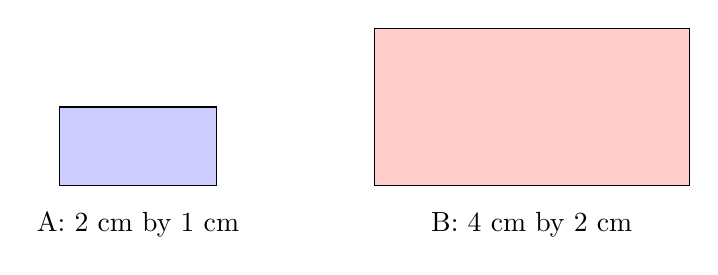
\begin{tikzpicture}
\draw[fill=blue!20] (0,0) rectangle (2,1);
\node at (1, -0.5) {A: 2 cm by 1 cm};
\draw[fill=red!20] (4,0) rectangle (8,2);
\node at (6, -0.5) {B: 4 cm by 2 cm};
\end{tikzpicture}
\end{center}

\vspace{1.2cm}

\item \begin{ealglossed}
A \ealgloss{square}{kwadrat} has a side length of \( s \). Another \ealgloss{square}{kwadrat} has a side length of \( 3s \). What is the \ealgloss{ratio}{stosunek} of the \ealgloss{perimeter}{obwodu} of the smaller \ealgloss{square}{kwadratu} to the larger \ealgloss{square}{kwadratu}? What is the \ealgloss{ratio}{stosunek} of their \ealgloss{areas}{pól}?
\end{ealglossed}

\vspace{1.2cm}

\item \begin{ealglossed}
A \ealgloss{right-angled triangle}{trójkąt prostokątny} has a \ealgloss{base}{podstawę} of 8 cm and a \ealgloss{height}{wysokość} of 6 cm. A \ealgloss{similar}{podobny} triangle has a \ealgloss{base}{podstawę} of 12 cm.
\end{ealglossed}
    \begin{enumerate}
    \item \begin{ealglossed}
    What is the \ealgloss{scale factor}{współczynnik skali} from the smaller to the larger triangle?
    \end{ealglossed}
    \item \begin{ealglossed}
    What is the \ealgloss{ratio}{stosunek} of the \ealgloss{perimeter}{obwodu} of the smaller triangle to the larger triangle?
    \end{ealglossed}
    \item \begin{ealglossed}
    What is the \ealgloss{ratio}{stosunek} of the \ealgloss{area}{pola} of the smaller triangle to the larger triangle?
    \end{ealglossed}
    \end{enumerate}

\vspace{1.2cm}

\newpage{}

\item \begin{ealglossed}
The diagram below shows a large rectangle with a smaller rectangle cut out of it. Find the \ealgloss{ratio}{stosunek} of the \ealgloss{area}{pola} of the shaded region to the \ealgloss{area}{pola} of the unshaded (cut-out) rectangle.
\end{ealglossed}

\vspace{0.5cm}
\begin{center}
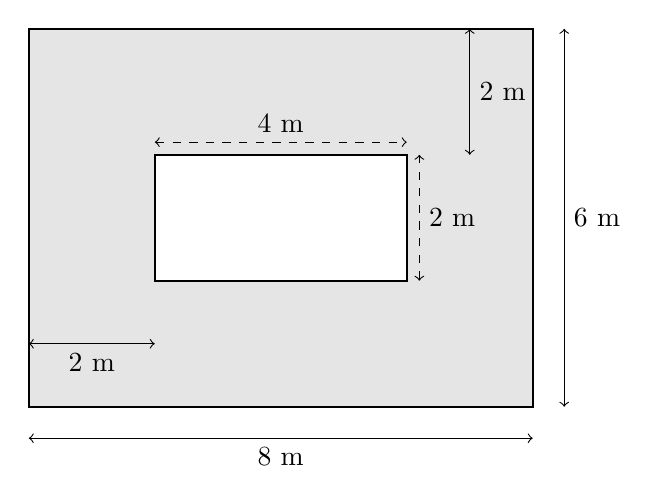
\begin{tikzpicture}[scale=0.8]
    % Big rectangle (shaded region)
    \fill[gray!20] (0,0) rectangle (8,6);
    \draw[thick] (0,0) rectangle (8,6);
    
    % Small rectangle (cut-out) - drawn with thicker white border to show cut-out effect
    \fill[white] (2,2) rectangle (6,4);
    \draw[thick, white] (2,2) rectangle (6,4);
    \draw[thick] (2,2) rectangle (6,4);
    
    % Labels for dimensions
    % Outer rectangle dimensions
    \draw[<->] (0,-0.5) -- (8,-0.5) node[midway,below] {8 m};
    \draw[<->] (8.5,0) -- (8.5,6) node[midway,right] {6 m};
    
    % Inner rectangle positioning dimensions
    \draw[<->] (0,1) -- (2,1) node[midway,below] {2 m};
    \draw[<->] (7,4) -- (7,6) node[midway,right] {2 m};
    
       
    % Inner rectangle dimensions
    \draw[<->, dashed] (2,4.2) -- (6,4.2) node[midway,above] {4 m};
    \draw[<->, dashed] (6.2,2) -- (6.2,4) node[midway,right] {2 m};
\end{tikzpicture}
\end{center}
\begin{ealglossed}
\textit{(\ealgloss{Dimensions}{Wymiary}: Large rectangle is 8m by 6m. The unshaded rectangle has a length of 4m and is positioned centrally.)}
\end{ealglossed}

\vspace{1.2cm}

\item \begin{ealglossed}
A circular pond has a \ealgloss{radius}{promień} of \( r \). A path is built around it, creating a larger circle with a \ealgloss{radius}{promieniu} of \( R \), where \( R = 2r \).
\end{ealglossed}
    \begin{enumerate}
    \item \begin{ealglossed}
    Find the \ealgloss{ratio}{stosunek} of the \ealgloss{circumference}{obwodu} of the pond to the \ealgloss{circumference}{obwodu} of the outer edge of the path.
    \end{ealglossed}
    \item \begin{ealglossed}
    Find the \ealgloss{ratio}{stosunek} of the \ealgloss{area}{pola} of the pond to the total \ealgloss{area}{pola} enclosed by the outer edge of the path.
    \end{ealglossed}
    \end{enumerate}

\vspace{1.2cm}
\end{enumerate}

\begin{ealglossed}
\section*{Sharing Into \ealgloss{Ratios}{stosunki} Past}
\end{ealglossed}
\begin{ealglossed}
Share the given quantities in the specified \ealgloss{ratios}{stosunkach}, using the \ealgloss{percentage}{procentowej} information to help you.
\end{ealglossed}

\begin{enumerate}
    \setcounter{enumi}{10}
    \item \begin{ealglossed}
    A sum of £80 is shared between two people. Person A receives 60\% of the total. What is the \ealgloss{ratio}{stosunek} of their shares, and how much does each person receive?
    \end{ealglossed}

    \item \begin{ealglossed}
    In a class, 40\% of students are boys and the rest are girls. The school fund of £150 is to be shared between boys and girls in the same \ealgloss{ratio}{stosunku} as their numbers in the class. How much do the boys get?
    \end{ealglossed}
    
    \item \begin{ealglossed}
    A bonus of £2,500 is shared between three departments in \ealgloss{proportion}{proporcjonalnie} to their \ealgloss{percentage}{procentowego} contribution to company profits. Department A contributed 25\%, Department B 35\%, and Department C the remainder. How much does each department receive, and what is the \ealgloss{ratio}{stosunek} of their shares in \ealgloss{simplest form}{najprostszej postaci}?
    \end{ealglossed}
    
    \item \begin{ealglossed}
    In a recipe, the dry ingredients (flour and sugar) are mixed in the \ealgloss{ratio}{stosunku} 3:2 by weight. If the flour makes up 30\% of the total mixture (including 400g of wet ingredients), find the weight of flour and sugar used.
    \end{ealglossed}
    
    \item \begin{ealglossed}
    An inheritance is shared between three children. The eldest receives 50\% of the total, the middle child receives 40\% of what the eldest gets, and the youngest receives the remaining £24,000. Find the total inheritance and the \ealgloss{ratio}{stosunek} of their shares in the form \textit{Eldest : Middle : Youngest}.
    \end{ealglossed}
\end{enumerate}



\begin{ealglossed}
\section*{Sharing Into \ealgloss{Ratios}{stosunki} Future}
\end{ealglossed}
Use the diagrams to help you solve the following problems.

\begin{enumerate}
    \setcounter{enumi}{15}
    \item \begin{ealglossed}
    The \ealgloss{perimeter}{obwód} of a rectangle is 30 cm. The sides are in the \ealgloss{ratio}{stosunku} 2:3. Find the \ealgloss{area}{pole} of the rectangle.
    \end{ealglossed}
    
    \item \begin{ealglossed}
    The \ealgloss{area}{pole} of a rectangle is 54 cm². The sides are in the \ealgloss{ratio}{stosunku} 2:3. Find the \ealgloss{perimeter}{obwód} of the rectangle.
    \end{ealglossed}
    

    \item \begin{ealglossed}
    A \ealgloss{right-angled triangle}{trójkąt prostokątny} has sides in the \ealgloss{ratio}{stosunku} 3:4:5. The \ealgloss{area}{pole} of the triangle is 96 cm². Find the \ealgloss{perimeter}{obwód} of the triangle.
    \end{ealglossed}
    
    \begin{tikzpicture}
        \draw (0,0) -- (4,0) -- (0,3) -- cycle;
        \node at (2, -0.3) {?};
        \node at (-0.3, 1.5) {?};
        \node at (2, 1.8) {?};
    \end{tikzpicture}

    \item \begin{ealglossed}
    A garden is in the shape of an L-shape made from two rectangles. The first rectangle is 3m by 2m. The second rectangle has sides in the \ealgloss{ratio}{stosunku} 3:4, If the total \ealgloss{area}{pole} of the garden is 54 m², find the \ealgloss{dimensions}{wymiary} of the second rectangle.
    \end{ealglossed}
    
    \begin{tikzpicture}[scale=0.5]
        \draw (0,0) rectangle (3,2);
        \draw (3,0) rectangle (7,4);
        \node at (1.5, -0.5) {3m};
        \node at (-0.55, 1) {2m};
        \node at (5, -0.5) {?};
        \node at (8, 2) {?};
    \end{tikzpicture}

    \newpage{}

    \item \begin{ealglossed}
    A circular pond is surrounded by a path. The \ealgloss{radius}{promień} of the pond and the width of the path are in the \ealgloss{ratio}{stosunku} 2:1. If the total \ealgloss{area}{pole} (pond + path) is $99\pi$m², find the width of the path.
    \end{ealglossed}
    
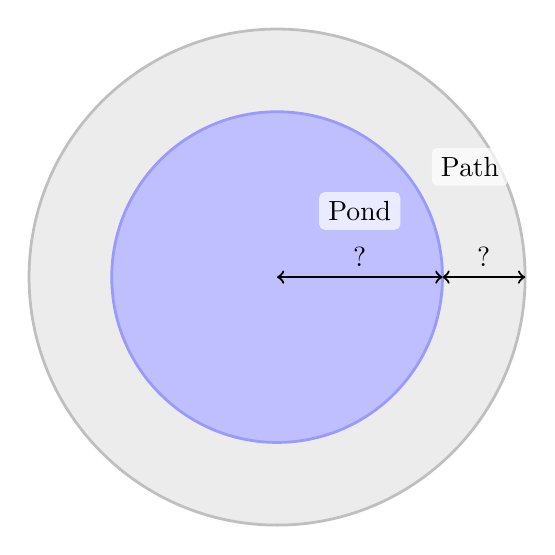
\begin{tikzpicture}[scale=0.7]
    % Path (annulus) - lighter fill with darker border
    \filldraw[fill=gray!15, draw=gray!50, line width=1pt] (0,0) circle (4.5);
    % Pond - darker fill with clear border
    \filldraw[fill=blue!25, draw=blue!40, line width=1pt] (0,0) circle (3);
    
    % Dimension lines with arrows and labels
    \draw[<->, line width=0.8pt] (0,0) -- (3,0) node[midway, above]{?};
    \draw[<->, line width=0.8pt] (3,0) -- (4.5,0) node[midway, above] {?};
    
    % Labels with better positioning and background
    \node[fill=white, fill opacity=0.7, text opacity=1, rounded corners=2pt] at (1.5, 1.2) {Pond};
    \node[fill=white, fill opacity=0.7, text opacity=1, rounded corners=2pt] at (3.5, 2.0) {Path};
    
\end{tikzpicture}
\end{enumerate}

\vspace{1cm}

\begin{ealglossed}
\section*{\ealgloss{Ratio}{stosunek} Problem Solving Past}
\end{ealglossed}
\begin{enumerate}[start=21]

    \item \begin{ealglossed}
    In a class, the \ealgloss{ratio}{stosunek} of boys to girls is $3:2$. 40\% of the boys wear glasses. 20\% of the girls wear glasses, what \ealgloss{percentage}{procent} of the \textit{whole class} wear glasses?
    \end{ealglossed}

    \item \begin{ealglossed}
    The price of a rare coin is increased by 20\%. The new \ealgloss{ratio}{stosunek} of its price to its original price is $a : b$. Write the \ealgloss{ratio}{stosunek} $a:b$ in its \ealgloss{simplest form}{najprostszej postaci}.
    \end{ealglossed}

    \item \begin{ealglossed}
    A shop sells only two types of fruit: apples and oranges. The \ealgloss{ratio}{stosunek} of apples to oranges is $5:3$. 30\% of the apples are green, and the rest are red. 60\% of the oranges are from Spain, and the rest are from Morocco. What is the \ealgloss{ratio}{stosunek} of \textbf{green apples} to \textbf{oranges from Morocco}?
    \end{ealglossed}

    \item \begin{ealglossed}
    In a library, the \ealgloss{ratio}{stosunek} of fiction to non-fiction books is $7:3$. After a donation, the number of fiction books increased by 15\% and the number of non-fiction books decreased by 10\%. Find the new \ealgloss{ratio}{stosunek} of fiction to non-fiction books. Give your answer in the form $A:B$ where $A$ and $B$ are \ealgloss{integers}{liczbami całkowitymi}.
    \end{ealglossed}

    \item \begin{ealglossed}
    The population of a town is 18,000. The \ealgloss{ratio}{stosunek} of adults to children is $5:4$. One year later, the adult population decreases by 5\% and the child population increases by 10\%.
    \end{ealglossed}
    \begin{enumerate}[label=(\alph*)]
        \item \begin{ealglossed}
        What is the new \ealgloss{ratio}{stosunek} of adults to children? Give your answer in its \ealgloss{simplest form}{najprostszej postaci}.
        \end{ealglossed}
        \item \begin{ealglossed}
        What is the overall \ealgloss{percentage}{procentowa} change in the total population? Give your answer to 2 decimal places.
        \end{ealglossed}
    \end{enumerate}

\end{enumerate}

\newpage{}


\begin{ealglossed}
\section*{\ealgloss{Ratio}{stosunek} Problem Solving Future}
\end{ealglossed}
\begin{enumerate}[start=26]

    \item \begin{ealglossed}
    Two rectangles, A and B, are \ealgloss{similar}{podobne}. The \ealgloss{ratio}{stosunek} of their \ealgloss{corresponding}{odpowiadających} lengths is $2:5$. What is the \ealgloss{ratio}{stosunek} of their \ealgloss{perimeters}{obwodów}? What is the \ealgloss{ratio}{stosunek} of their \ealgloss{areas}{pól}?
    \end{ealglossed}

    \item \begin{ealglossed}
    A rectangle has a length to width \ealgloss{ratio}{stosunek} of $5:2$. Its \ealgloss{perimeter}{obwód} is 42 cm.
    \end{ealglossed}
    \begin{enumerate}[label=(\alph*)]
        \item \begin{ealglossed}
        Find its \ealgloss{area}{pole}.
        \end{ealglossed}
        \item \begin{ealglossed}
        If the rectangle is \ealgloss{enlarged}{powiększany} by a \ealgloss{scale factor}{współczynnik skali} of 3, what is the new \ealgloss{ratio}{stosunek} of length to width, and what is its new \ealgloss{area}{pole}?
        \end{ealglossed}
    \end{enumerate}

    \item \begin{ealglossed}
    The \ealgloss{ratio}{stosunek} of the \ealgloss{area}{pola} of a \ealgloss{square}{kwadratu} to the \ealgloss{area}{pola} of an \ealgloss{equilateral triangle}{trójkąta równobocznego} is $16:9$. The \ealgloss{perimeter}{obwód} of the \ealgloss{square}{kwadratu} is 32 cm. What is the length of one side of the triangle?
    \end{ealglossed}

    \item \begin{ealglossed}
    The \ealgloss{perimeter}{obwód} of an \ealgloss{isosceles triangle}{trójkąta równoramiennego} is 36 cm. The \ealgloss{ratio}{stosunek} of the equal sides to the \ealgloss{base}{podstawy} is $5:2$.
    \end{ealglossed}
    \begin{enumerate}[label=(\alph*)]
        \item Calculate the lengths of the sides of the triangle.
        \item \begin{ealglossed}
        Calculate the \ealgloss{area}{pole} of the triangle. (Hint: You may need to use \ealgloss{Pythagoras' Theorem}{twierdzenia Pitagorasa} - ask your teacher to help you draw a picture!).
        \end{ealglossed}
    \end{enumerate}

    \item \begin{ealglossed}
    The diagram below shows a large rectangle, measuring 20 cm at the \ealgloss{base}{podstawy}, with a \ealgloss{similar}{podobnym} smaller rectangle, \ealgloss{height}{wysokości} 4 cm cut out from one corner. The \ealgloss{ratio}{stosunek} of the length to the width of the smaller rectangle is the same as the \ealgloss{ratio}{stosunek} of the length to the width of the large rectangle.
    \end{ealglossed}
    
    \begin{center}
    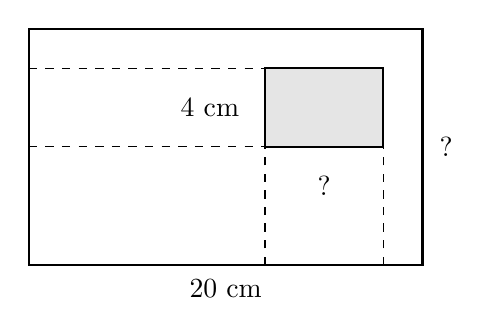
\begin{tikzpicture}
        \draw[thick] (0,0) rectangle (5,3);
        \draw[thick, fill=gray!20] (3,1.5) rectangle (4.5,2.5);
        \draw[dashed] (3,0) -- (3,1.5);
        \draw[dashed] (4.5,0) -- (4.5,1.5);
        \draw[dashed] (0,1.5) -- (3,1.5);
        \draw[dashed] (0,2.5) -- (3,2.5);
        \node at (2.5, -0.3) {20 cm};
        \node at (5.3, 1.5) {?};
        \node at (2.3, 2) {4 cm};
        \node at (3.75, 1) {?};
    \end{tikzpicture}
    \end{center}
    
    \begin{ealglossed}
    Given that the \ealgloss{area}{pole} of the large rectangle with the small one cut out is $216 \text{ cm}^2$, find the \ealgloss{dimensions}{wymiary} of the smaller rectangle.
    \end{ealglossed}

\end{enumerate}

\end{document}